\documentclass{article}%
\usepackage[T1]{fontenc}%
\usepackage[utf8]{inputenc}%
\usepackage{lmodern}%
\usepackage{textcomp}%
\usepackage{lastpage}%
\usepackage{geometry}%
\geometry{margin=1in}%
\usepackage{tikz}%
\usepackage{pgfplots}%
\pgfplotsset{compat=1.18}%
\usepackage{booktabs}%
\usepackage{caption}%
\usepackage{siunitx}%
\usepackage{graphicx}%
%
\graphicspath{{../assets/}}%
\title{Simply Supported Beam Analysis Report}%
\author{Automated PyLaTeX Generator}%
\date{\today}%
%
\begin{document}%
\normalsize%
\maketitle%
\tableofcontents\newpage%
\section{Introduction}%
\label{sec:Introduction}%
This report presents a simple structural analysis of a simply supported beam subjected to point loads. The reactions, shear force diagram (SFD), and bending moment diagram (BMD) are computed and plotted using pgfplots.

%
\section{Beam Description}%
\label{sec:BeamDescription}%
Beam supports: simple supports at x=0 and x=L. Units are consistent (e.g., meters and Newtons).%


\begin{figure}[h!]%
\centering%
\includegraphics[width=0.8\textwidth]{beam.png}%
\caption{Simply supported beam schematic}%
\end{figure}

%
\section{Data Source}%
\label{sec:DataSource}%
Input data read from the Excel file data/forces.xlsx. The following table reproduces the input data used for analysis.

%
\section{Input Data}%
\label{sec:InputData}%
\captionof{table}{Input data read from Excel (X, Shear, Bending Moment)}%
\begin{tabular}{lrr}%
\toprule%
\textbf{X (m)}&\textbf{Shear (N)}&\textbf{Moment (N\,m)}\\%
\midrule%
0.000&5.000&0.000\\%
0.100&4.900&0.497\\%
0.200&4.800&0.990\\%
0.300&4.700&1.478\\%
0.400&4.600&1.960\\%
0.500&4.500&2.438\\%
0.600&4.400&2.910\\%
0.700&4.300&3.377\\%
0.800&4.200&3.840\\%
0.900&4.100&4.298\\%
1.000&4.000&4.750\\%
1.100&3.900&5.197\\%
1.200&3.800&5.640\\%
1.300&3.700&6.077\\%
1.400&3.600&6.510\\%
1.500&3.500&6.938\\%
1.600&3.400&7.360\\%
1.700&3.300&7.777\\%
1.800&3.200&8.190\\%
1.900&3.100&8.598\\%
2.000&3.000&9.000\\%
2.100&2.900&9.398\\%
2.200&2.800&9.790\\%
2.300&2.700&10.178\\%
2.400&2.600&10.560\\%
2.500&2.500&10.938\\%
2.600&2.400&11.310\\%
2.700&2.300&11.678\\%
2.800&2.200&12.040\\%
2.900&2.100&12.398\\%
3.000&2.000&12.750\\%
3.100&1.900&13.098\\%
3.200&1.800&13.440\\%
3.300&1.700&13.777\\%
3.400&1.600&14.110\\%
3.500&1.500&14.438\\%
3.600&1.400&14.760\\%
3.700&1.300&15.078\\%
3.800&1.200&15.390\\%
3.900&1.100&15.697\\%
4.000&1.000&16.000\\%
4.100&0.900&16.297\\%
4.200&0.800&16.590\\%
4.300&0.700&16.878\\%
4.400&0.600&17.160\\%
4.500&0.500&17.438\\%
4.600&0.400&17.710\\%
4.700&0.300&17.977\\%
4.800&0.200&18.240\\%
4.900&0.100&18.497\\%
5.000&0.000&18.750\\%
5.100&{-}0.100&18.997\\%
5.200&{-}0.200&19.240\\%
5.300&{-}0.300&19.477\\%
5.400&{-}0.400&19.710\\%
5.500&{-}0.500&19.938\\%
5.600&{-}0.600&20.160\\%
5.700&{-}0.700&20.378\\%
5.800&{-}0.800&20.590\\%
5.900&{-}0.900&20.797\\%
6.000&{-}1.000&21.000\\%
6.100&{-}1.100&21.198\\%
6.200&{-}1.200&21.390\\%
6.300&{-}1.300&21.578\\%
6.400&{-}1.400&21.760\\%
6.500&{-}1.500&21.938\\%
6.600&{-}1.600&22.110\\%
6.700&{-}1.700&22.277\\%
6.800&{-}1.800&22.440\\%
6.900&{-}1.900&22.598\\%
7.000&{-}2.000&22.750\\%
7.100&{-}2.100&22.898\\%
7.200&{-}2.200&23.040\\%
7.300&{-}2.300&23.177\\%
7.400&{-}2.400&23.310\\%
7.500&{-}2.500&23.438\\%
7.600&{-}2.600&23.560\\%
7.700&{-}2.700&23.677\\%
7.800&{-}2.800&23.790\\%
7.900&{-}2.900&23.898\\%
8.000&{-}3.000&24.000\\%
8.100&{-}3.100&24.098\\%
8.200&{-}3.200&24.190\\%
8.300&{-}3.300&24.277\\%
8.400&{-}3.400&24.360\\%
8.500&{-}3.500&24.438\\%
8.600&{-}3.600&24.510\\%
8.700&{-}3.700&24.578\\%
8.800&{-}3.800&24.640\\%
8.900&{-}3.900&24.698\\%
9.000&{-}4.000&24.750\\%
9.100&{-}4.100&24.797\\%
9.200&{-}4.200&24.840\\%
9.300&{-}4.300&24.878\\%
9.400&{-}4.400&24.910\\%
9.500&{-}4.500&24.938\\%
9.600&{-}4.600&24.960\\%
9.700&{-}4.700&24.977\\%
9.800&{-}4.800&24.990\\%
9.900&{-}4.900&24.997\\%
10.000&{-}5.000&25.000\\%
\bottomrule%
\end{tabular}

%
\section{Analysis}%
\label{sec:Analysis}%
The following diagrams are generated directly from the provided Excel data. Reactions and load inference were not computed; the supplied SFD and BMD are used as{-}is.%
\subsection{Shear Force Diagram (SFD)}%
\label{subsec:ShearForceDiagram(SFD)}%

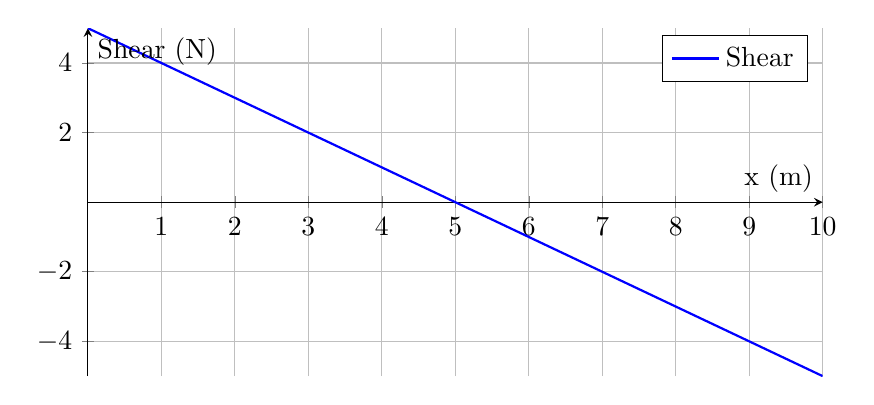
\begin{tikzpicture}
  \begin{axis}[
    width=0.9\textwidth,
    height=6cm,
    xlabel={x (m)},
    ylabel={Shear (N)},
    grid=both,
    axis lines=middle,
  ]
    \addplot+[no markers, thick] coordinates {
            (0.000,5.000)
            (0.100,4.900)
            (0.200,4.800)
            (0.300,4.700)
            (0.400,4.600)
            (0.500,4.500)
            (0.600,4.400)
            (0.700,4.300)
            (0.800,4.200)
            (0.900,4.100)
            (1.000,4.000)
            (1.100,3.900)
            (1.200,3.800)
            (1.300,3.700)
            (1.400,3.600)
            (1.500,3.500)
            (1.600,3.400)
            (1.700,3.300)
            (1.800,3.200)
            (1.900,3.100)
            (2.000,3.000)
            (2.100,2.900)
            (2.200,2.800)
            (2.300,2.700)
            (2.400,2.600)
            (2.500,2.500)
            (2.600,2.400)
            (2.700,2.300)
            (2.800,2.200)
            (2.900,2.100)
            (3.000,2.000)
            (3.100,1.900)
            (3.200,1.800)
            (3.300,1.700)
            (3.400,1.600)
            (3.500,1.500)
            (3.600,1.400)
            (3.700,1.300)
            (3.800,1.200)
            (3.900,1.100)
            (4.000,1.000)
            (4.100,0.900)
            (4.200,0.800)
            (4.300,0.700)
            (4.400,0.600)
            (4.500,0.500)
            (4.600,0.400)
            (4.700,0.300)
            (4.800,0.200)
            (4.900,0.100)
            (5.000,0.000)
            (5.100,-0.100)
            (5.200,-0.200)
            (5.300,-0.300)
            (5.400,-0.400)
            (5.500,-0.500)
            (5.600,-0.600)
            (5.700,-0.700)
            (5.800,-0.800)
            (5.900,-0.900)
            (6.000,-1.000)
            (6.100,-1.100)
            (6.200,-1.200)
            (6.300,-1.300)
            (6.400,-1.400)
            (6.500,-1.500)
            (6.600,-1.600)
            (6.700,-1.700)
            (6.800,-1.800)
            (6.900,-1.900)
            (7.000,-2.000)
            (7.100,-2.100)
            (7.200,-2.200)
            (7.300,-2.300)
            (7.400,-2.400)
            (7.500,-2.500)
            (7.600,-2.600)
            (7.700,-2.700)
            (7.800,-2.800)
            (7.900,-2.900)
            (8.000,-3.000)
            (8.100,-3.100)
            (8.200,-3.200)
            (8.300,-3.300)
            (8.400,-3.400)
            (8.500,-3.500)
            (8.600,-3.600)
            (8.700,-3.700)
            (8.800,-3.800)
            (8.900,-3.900)
            (9.000,-4.000)
            (9.100,-4.100)
            (9.200,-4.200)
            (9.300,-4.300)
            (9.400,-4.400)
            (9.500,-4.500)
            (9.600,-4.600)
            (9.700,-4.700)
            (9.800,-4.800)
            (9.900,-4.900)
            (10.000,-5.000)
    };
    \addlegendentry{Shear}
  \end{axis}
\end{tikzpicture}

%
\subsection{Bending Moment Diagram (BMD)}%
\label{subsec:BendingMomentDiagram(BMD)}%

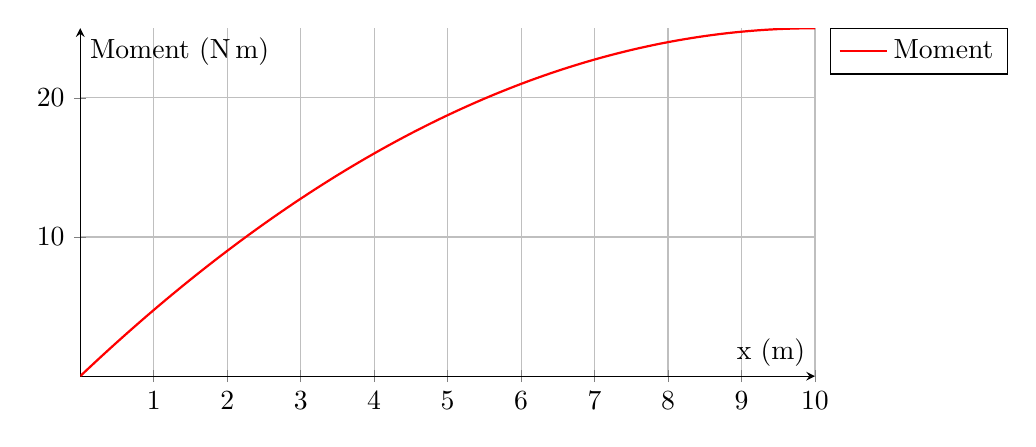
\begin{tikzpicture}
    \begin{axis}[
        width=0.9\textwidth,
        height=6cm,
        xlabel={x (m)},
        ylabel={Moment (N\,m)},
        grid=both,
        axis lines=middle,
        legend style={at={(1.02,1)},anchor=north west},
    ]
    \addplot+[no markers, thick, color=red] coordinates {
            (0.000,0.000)
            (0.100,0.497)
            (0.200,0.990)
            (0.300,1.478)
            (0.400,1.960)
            (0.500,2.438)
            (0.600,2.910)
            (0.700,3.377)
            (0.800,3.840)
            (0.900,4.298)
            (1.000,4.750)
            (1.100,5.197)
            (1.200,5.640)
            (1.300,6.077)
            (1.400,6.510)
            (1.500,6.938)
            (1.600,7.360)
            (1.700,7.777)
            (1.800,8.190)
            (1.900,8.598)
            (2.000,9.000)
            (2.100,9.398)
            (2.200,9.790)
            (2.300,10.178)
            (2.400,10.560)
            (2.500,10.938)
            (2.600,11.310)
            (2.700,11.678)
            (2.800,12.040)
            (2.900,12.398)
            (3.000,12.750)
            (3.100,13.098)
            (3.200,13.440)
            (3.300,13.777)
            (3.400,14.110)
            (3.500,14.438)
            (3.600,14.760)
            (3.700,15.078)
            (3.800,15.390)
            (3.900,15.697)
            (4.000,16.000)
            (4.100,16.297)
            (4.200,16.590)
            (4.300,16.878)
            (4.400,17.160)
            (4.500,17.438)
            (4.600,17.710)
            (4.700,17.977)
            (4.800,18.240)
            (4.900,18.497)
            (5.000,18.750)
            (5.100,18.997)
            (5.200,19.240)
            (5.300,19.477)
            (5.400,19.710)
            (5.500,19.938)
            (5.600,20.160)
            (5.700,20.378)
            (5.800,20.590)
            (5.900,20.797)
            (6.000,21.000)
            (6.100,21.198)
            (6.200,21.390)
            (6.300,21.578)
            (6.400,21.760)
            (6.500,21.938)
            (6.600,22.110)
            (6.700,22.277)
            (6.800,22.440)
            (6.900,22.598)
            (7.000,22.750)
            (7.100,22.898)
            (7.200,23.040)
            (7.300,23.177)
            (7.400,23.310)
            (7.500,23.438)
            (7.600,23.560)
            (7.700,23.677)
            (7.800,23.790)
            (7.900,23.898)
            (8.000,24.000)
            (8.100,24.098)
            (8.200,24.190)
            (8.300,24.277)
            (8.400,24.360)
            (8.500,24.438)
            (8.600,24.510)
            (8.700,24.578)
            (8.800,24.640)
            (8.900,24.698)
            (9.000,24.750)
            (9.100,24.797)
            (9.200,24.840)
            (9.300,24.878)
            (9.400,24.910)
            (9.500,24.938)
            (9.600,24.960)
            (9.700,24.977)
            (9.800,24.990)
            (9.900,24.997)
            (10.000,25.000)
    };
    \addlegendentry{Moment}
  \end{axis}
\end{tikzpicture}

%
\subsection{Summary}%
\label{subsec:Summary}%
Key results:%
Maximum shear: 5.000 N at x = 0.000 m\\%
Maximum moment: 25.000 N\,m at x = 10.000 m\\%
\newline%
%
A Shear Force Diagram (SFD) represents the internal shear force distribution along the beam as a function of position. It shows how shear changes where loads are applied and at supports; abrupt jumps correspond to point loads or reactions.%
\newline%
\newline%
%
A Bending Moment Diagram (BMD) represents the internal bending moment distribution along the beam. It indicates where the beam experiences the largest bending effects; these locations are critical for section design and checks.

%
\end{document}